% !Mode:: "TeX:UTF-8"
\chapter{解决路径规划问题的其他优化算法}
除了使用Hopfield神经网络解决路劲规划问题外,我们下面介绍另外几种常用于解决路径规划的算法。
\section{暴力穷举搜索}
穷举法是解决该问题的最简单的一种算法,它为了达到求解的目的,利用计算机强大的算力来寻找与比较各个可行解,
但是,穷举算法在城市数量较多时效率不高。下面是对待路径规划问题上的穷举算法流程图:\\
\begin{figure}[H]
    \centering
    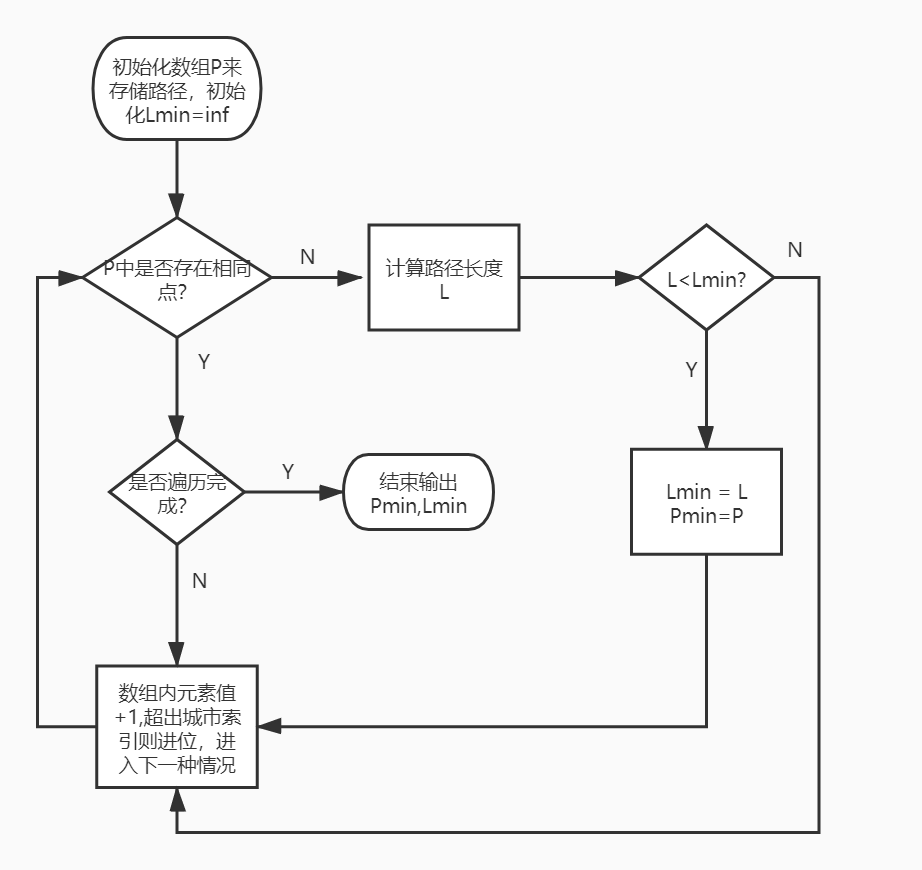
\includegraphics[width=13cm]{figure/blqj.jpg}
    \caption{暴力穷举搜索流程图}
    \label{fig-blqj}%暴力穷举
\end{figure}
\par
其中$P=[p_1,p_2,\cdots,p_n]$为存储路径的数组,城市的标号为$\{1,2,3,\cdots, n\}$,P遍历为下一种路径的方法为,$p_n + 1$,若$p_n = n$则$p_{n-1}+1,p_n=1$,以此类推,遍历得到解空间所有路径集合。
\section{剪枝法}
经典剪枝法进行改进,利用启发式算法来估计解空间树某一结点的剩余部分的所代表的路径代价,首先先介绍最近邻点算法(nearest neighbor heuristic),该算法的具体步骤如下所示:
\par
$Step \quad 1: \quad $任选点$r \in V$起点, 令$C={r},h=r$。
\par
$Step \quad 2: \quad $找到下一个相邻点,该点满足$k \in V \backslash C $使得$C_{hk}=min\{c_{hj}, c_{jh}\}$,将$k$加入$C$中。
\par
$Step \quad 3: \quad $当$|C|=|V|$算法终止,否则$h=k$则返回$Step \quad 2$。
\par
我们将最近邻点算法来估计路径剩余部分的花费。所以,剪枝法的算法流程图修改如下:
\begin{figure}[H]
    \centering
    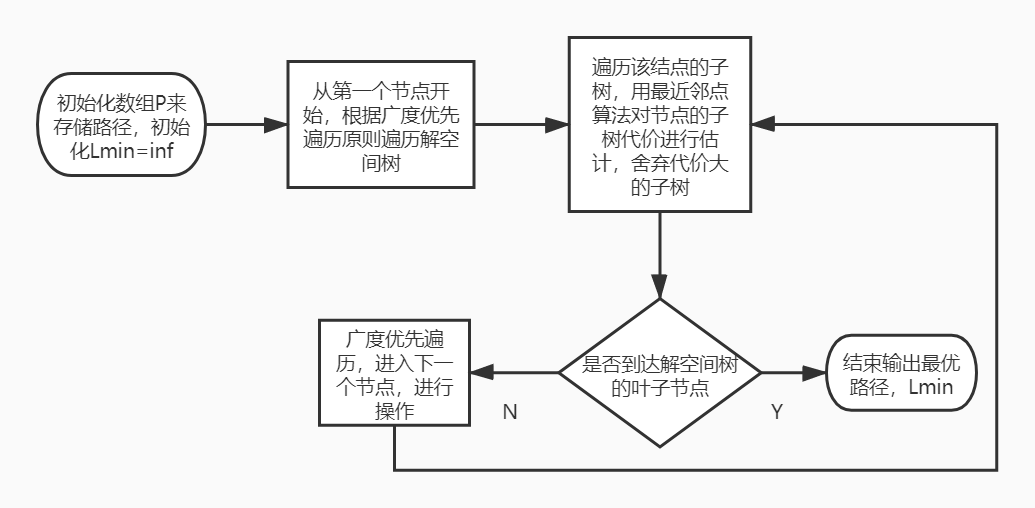
\includegraphics[width=13cm]{figure/qfsjzf.jpg}%启发式剪枝法
    \caption{利用启发式算法的剪枝法解决TSP问题算法流程图}
    \label{fig-qfsjzf}
\end{figure}
\section{智能算法简介}
\subsection{粒子群算法}
粒子群算法(particle swarm optimization, PSO)是一种群体智能的优化算法,和蚁群算法,鱼群算法一样。该算法思想来源于鸟类捕猎的行为,即鸟群捕食时最有效的是搜索离目标最近的鸟的区域。
算法首先随机一群粒子,根据每个粒子对应的适应度函数来决定该粒子的移动方向与距离。\\
假设粒子$x_i$在空间的位置为$x_i = \{x_1,x_2,\cdots, x_n\}$初始速度为$v_i = \{v_1,v_2,\cdots, v_n\}$,每个粒子已知自己经过的最好位置与现在位置,还知道群体的最好位置。则速度与位置的更新规则如下:
\begin{align}
    v_i = \omega \times v_i + c_1 \times rand() \times (pbest_i - x_i) + c_2 \times rand() \times (gbest_i - x_i)
\end{align}
其中上式$\omega$被称为惯性因子,其值较大时,全局寻优能力强,但局部寻优能力弱,当此值较小时,全局寻优能力弱,局部寻优能力强,但其值大于零。在算法实现时动态的$\omega$可能会有更好的效果。目前采用的时线性递减权值策略(Linearly Decreasing Weight, LDW):
\begin{align}
    \omega^{(t)} = \frac{(\omega_{ini} - \omega_{end})(G_k - g)}{G_k} + \omega_{end}
\end{align}
上式中$G_k$代表最大迭代次数,$\omega_{ini}$代表初始惯性权值,$\omega_{end}$表示迭代到最大进化次数时的惯性权值。\\
下面给出$PSO$算法流程图:
\begin{figure}[H]
    \centering
    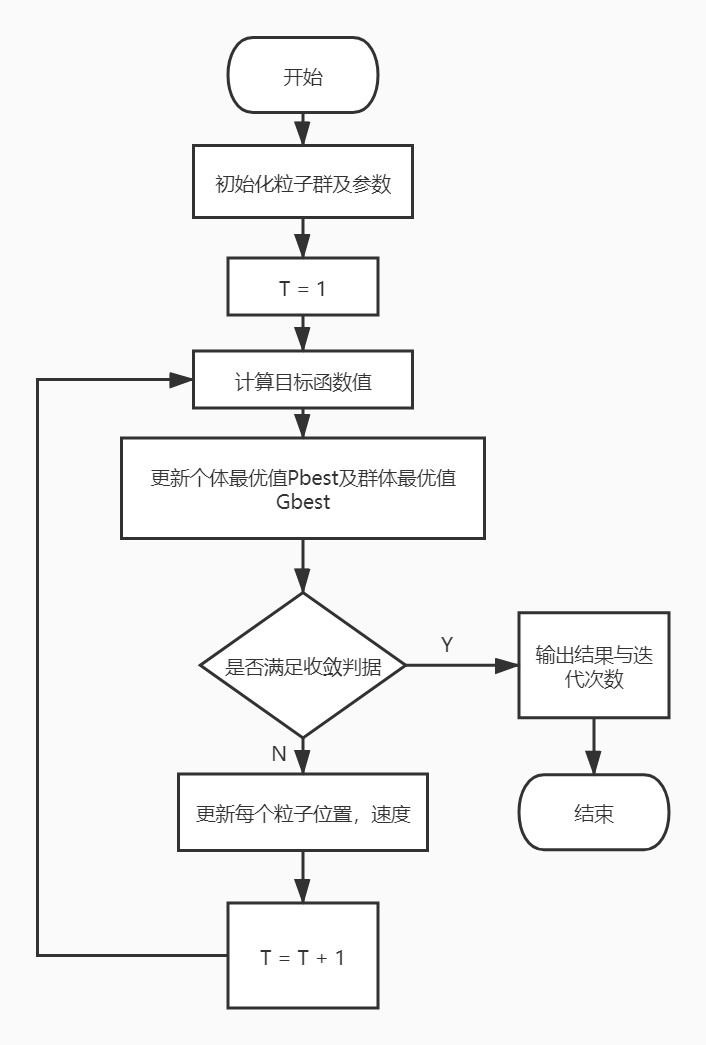
\includegraphics[width=13cm]{figure/PSO.jpg}%启发式剪枝法
    \caption{粒子群算法流程图}
    \label{fig-pso}
\end{figure}
\subsection{模拟退火算法}
统计力学证明了物质的粒子不同结构对应于粒子的不同能量水平,高温下粒子可以自由活动,低温下粒子的活动渐渐减弱,所以从高温开始降温,
粒子可以在每个温度达到某种平衡,我们称为粒子热平衡,我们称这种行为为退火。系统降温到被冷却时,材料成为了低能状态下的晶体。根据此现象,研究人员发明创立了模拟退火算法。
\par
$Metropllis$算法用数学模型描述了材料退火的过程。$E(i)$为i状态下的能量,即材料的状态转换遵循如下规律:
\par
(1) 若$E(j) \le E(i) $,状态转换。
\par
(2) 若$E(j) > E(i)$,状态以一定概率改变,即$\frac{E(i)-E(j)}{KT}$。其中$K$为玻尔兹曼常数常应用于物理学领域,$T$为材料温度。
下面我们将退火思想移植到优化问题上来。以组合优化问题为例,设
目标函数为$f:x \rightarrow R_{+},x \in S,R_{+} = \{y|y \in R,y > 0\}$,$N(x) \subseteq S$代表$S$代表定义域。
\par
设该问题的初始温度为$T_0$,初始解为$x(0)$,以及由初始解生成的下一个解$x^{'} \in N(x(0))$:
\begin{align}
    P\left(x(0) \rightarrow x^{\prime}\right)=\left\{\begin{array}{ll}
        1 & \text { 若 } f\left(x^{\prime}\right)<f(x(0)) \\
        e^{-\frac{f\left(x^{'}\right)-f(x(0))}{T_{0}}} & \text { 其它 }
        \end{array}\right.
\end{align}
其中$P\left(x(0) \rightarrow x^{\prime}\right)$代表$x^{'}$是否为新解的概率。上式可以这么解释,即若$x^{'}$的函数值比上一个解小,则$x^{'}$必定为新解,否则以一定概率作为新解。
\par
将此式推广则可以得到:
\begin{align}
    P\left(x(0) \rightarrow x^{\prime}\right)=\left\{\begin{array}{ll}
        1 & \text { 若 } f\left(x^{\prime}\right)<f(x(k)) \\
        e^{-\frac{f\left(x^{'}\right)-f(x(k))}{T_{k}}} & \text { 其它 }
        \end{array}\right.
        \label{thddgs}%退火迭代公式
\end{align}
若重复多次该过程即为不断求得新解且系统逐渐降温的过程。在每个$T_i$下每个新状态$x(k+1)$依赖于前一个状态,且于前$k-1$个状态无关,这是一个马尔可夫过程,
\par
模拟退火算法在计算机实现时可能会出现如下问题:
1.降温过慢,找到优质解的概率较大,但时间较长,降温过快,找到优质解的概率较小,但时间较短,所以在实现过程中要兼顾速度与性能。
2.若连续多次转换都没有使得状态改变则改变该温度,程序结束条件可以为,连续几个温度下状态都没有发生转变。
3.初值的选取会影响程序的性能与解的质量。
\subsection{遗传算法}
遗传算法(Genetic Algorithms,GA)是一种搜索算法,他的思想来源于自然选择,与遗传进化。模拟自然界的选择机制,对优化目标进行寻优求解 ,算法与自然界的遗传选择之间的对应关系为:
适者生存具体表现为每次算法迭代完成一次后都会最大可能的留住最优解淘汰劣质解,算法中的每个个体都代表一个解,解在算法中被编码对应了染色体,其基因代表,解的每个分量,个体适应度,具体体现在目标函数上,交配根据交换优质解的特征来生成其他解,变异,改变解的某一分量以扩大搜索范围,它在算法实现方面主要分为6部分,
1.种群初始化,
2.构造适应度函数,
3.选择操作,
4.交叉操作,
5.变异操作,
6.寻优;
遗传算法解决优化问题的算法流程如下,以非线性优化为例:
\begin{figure}[H]
    \centering
    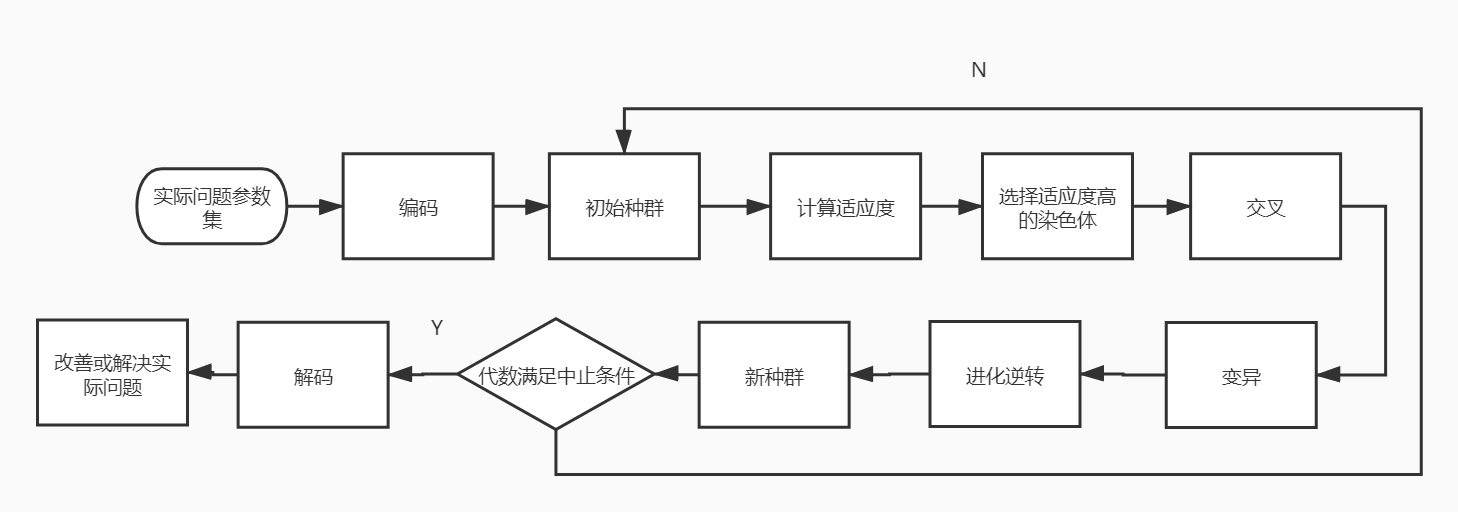
\includegraphics[width=13cm]{figure/ycsf.jpg}%启发式剪枝法
    \caption{遗传算法流程图}
    \label{fig-ycsf}
\end{figure}
\subsection{蚁群算法}
1991年来自意大利的学者M. Dorigo 首先提出了蚁群算法,人么并以此为基础逐渐发展完善了蚁群算法,科学家们发现蚂蚁会在路上释放挥发性的信息素,蚂蚁个体之间就是通过这种信息素进行交流,蚂蚁总是趋向于走更多信息素的路径,假设最短路径的蚂蚁回到了巢穴因为其路径最短时间最优,所以他的路径下的信息素浓度最高,所以走最短路径的蚂蚁会越来越多,以此形成正反馈,所有的蚂蚁都会趋于这条路径。
以解决TSP问题为例,$n$表示城市数量,$m$表示蚁群的蚂蚁数量,$d_{ij}$表示$i,j$城市之间的距离,$b_i(t)$表示在$t$时刻位于城市$i$的蚂蚁的个数。$m = \sum_{i=1}^n b_i(t)$;$\tau_{ij}(t)$为t时刻i到j的信息素浓度,其初值为常数,$\eta_{ij}(t)$表示t时刻i到j城市的转移期望。但人工蚁群中植入了记忆功能,随着时间推移信息素浓度会减少。
蚁群算法步骤可以被总结为:
\par
$Step \quad 1: \quad $初始化迭代次数,个参数初始化,蚁群位置初始化
\par
$Step \quad 2: \quad $对于每个蚂蚁威威按概率$p_{ij}^{k}$进行更新。
\par
$Step \quad 3: \quad $计算蚁群中每个个体的目标函数值,记录最优解。
\par
$Step \quad 4: \quad $更新信息素浓度。
\par
$Step \quad 5: \quad $迭代次数加一,若达到预定迭代次数则退出,否则转$Step \quad 2$。\\
\section{动态规划}
动态规划(dynamic programming)通过将待求解的问题划分为子问题的方法来求解。与将问题划分为互不相交的子问题然后递归的求解子问题的分治算法不同,动态规划不同它应用于子问题重叠的情况,子问题递归求解,再将其划分为更小的问题,
我们将其称为子子问题,子子问题在动态规划中只会被求解一次而在分治算法中会被重复求解,因为动态规划会将解存到一个表格中,避免了重复运算。我们将动态规划具体分为四个步骤:\\
\par
$Step \quad 1: \quad $构造并寻找解的结构。
\par
$Step \quad 2: \quad $递归的定义解。
\par
$Step \quad 3: \quad $自底向上的求解问题的解。
\par
$Step \quad 4: \quad $利用已知信息得到最优解。
下面我们来推导TSP问题的动态规划方程:\\
我们将问题划分为以下几种情况:
\par
(1)若$V^{'}$为空是,则$d(i,V^{'})$表示点$i$直接回到了原点。
\par
(2)若$V^{'}$不为空,则$d(i,V^{'})$代表了对子问题的最优解,程序中会在$V^{'}$的集合中逐一尝试最终得到最优解:
所以TSP问题的动态规划方程如下:
\begin{align}
    d(i, V)=\left\{\begin{array}{ll}c_{i s} & V=\phi, i \neq s \\\min _{h c r}\left\{c_{i k}+d(k, V-\{k\})\right\} & V \neq \phi\end{array}\right.
\end{align}

